\documentclass[addpoints]{exam}

%\printanswers
\noprintanswers

\usepackage{amsmath,bigstrut,minted,url,graphicx}

\pagestyle{headandfoot}
\runningheadrule
\firstpageheader{}{}{Page \thepage\ of \numpages}
\runningheader{CS 321}{Sample Problems}{Page \thepage\ of \numpages}
\firstpagefooter{}{}{}
\runningfooter{}{}{}
              
\begin{document}

\begin{center}
{\Large \textbf{
    Ozyegin University\\
    CS 321 Programming Languages\\
    Sample Problems on Functional Programming
}}
\end{center}

\begin{questions}
  \question
  Given the following OCaml code.
  \begin{minted}{ocaml}
    let x = 3;;
    let f y = x * y;;
    let x = 5;;
    let z = f 2;;
    let k = f x;;
    x = 10;;
    let w = f x;;
    let x = "hi";;
  \end{minted}
  
  \begin{parts}
    \part What are the values of \texttt{z}, \texttt{k}, and \texttt{w}?
    \begin{solutionbox}{1cm}
      6, 15, 15
    \end{solutionbox}
    
    \part Does the last line cause a type error?
    If not, what is the final value of \texttt{x}?
    \begin{solutionbox}{1cm}
      No error. The value is \verb|"hi"|.
    \end{solutionbox}
  \end{parts}


  \question
  Consider the following OCaml program:
  \begin{minted}{ocaml}
    let a = 5
    in (let b = 3 in a + b) + (let b = 9 in a * b)
  \end{minted}
  Assuming we start with the empty environment,
  \begin{parts}
    \part what's the environment in which the expression \mintinline{ocaml}{a + b}
    is evaluated?
    \begin{solutionbox}{1cm}
      [b $\mapsto$ 3, a $\mapsto$ 5]
    \end{solutionbox}

    \part what's the environment in which the expression \mintinline{ocaml}{a * b}
    is evaluated?
    \begin{solutionbox}{1cm}
      [b $\mapsto$ 9, a $\mapsto$ 5]
    \end{solutionbox}

    \part what's the environment after the expression is evaluated?
    \begin{solutionbox}{1cm}
      [~]
    \end{solutionbox}

    \part what does the expression evaluate to?
    \begin{solutionbox}{1cm}
      53
    \end{solutionbox}
  \end{parts}

  \question
  Consider the following OCaml program:
  \begin{minted}{ocaml}
    (let c = 3 in c + c) + (let c = 9 in c * c)
  \end{minted}
  Assuming we start with the empty environment,
  \begin{parts}
    \part what's the environment in which the expression \mintinline{ocaml}{c + c}
    is evaluated?
    \begin{solutionbox}{1cm}
      [c $\mapsto$ 3]
    \end{solutionbox}

    \part what's the environment in which the expression \mintinline{ocaml}{c * c}
    is evaluated?
    \begin{solutionbox}{1cm}
      [c $\mapsto$ 5]
    \end{solutionbox}

    \part what's the environment after the expression is evaluated?
    \begin{solutionbox}{1cm}
      [~]
    \end{solutionbox}

    \part what does the expression evaluate to?
    \begin{solutionbox}{1cm}
      87
    \end{solutionbox}
  \end{parts}
  

  \question
  Consider the following OCaml program:

  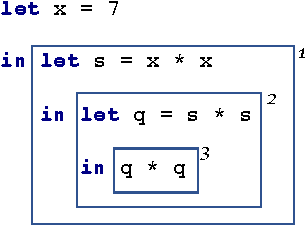
\includegraphics[width=5cm]{env1.pdf}
  
  Assuming we start with the empty environment,
  \begin{parts}
    \part what's the environment in which expression 1 is evaluated?
    \begin{solutionbox}{1cm}
      [x $\mapsto$ 7]
    \end{solutionbox}

    \part what's the environment in which expression 2 is evaluated?
    \begin{solutionbox}{1cm}
      [s $\mapsto$ 49, x $\mapsto$ 7]
    \end{solutionbox}

    \part what's the environment in which the expression \mintinline{ocaml}{s * s} is evaluated?
    \begin{solutionbox}{1cm}
      [s $\mapsto$ 49, x $\mapsto$ 7]
    \end{solutionbox}

    \part what's the environment in which expression 3 is evaluated?
    \begin{solutionbox}{1cm}
      [q $\mapsto$ 2401, s $\mapsto$ 49, x $\mapsto$ 7]
    \end{solutionbox}
  \end{parts}

  \question
  Consider the following OCaml program:
  \begin{minted}{ocaml}
    let x =
      let a = 5
      in let b = 8
         in a + b
    in x * 2
  \end{minted}
  Assuming we start with the empty environment,
  \begin{parts}
    \part what's the environment in which the expression \mintinline{ocaml}{a + b}
    is evaluated?
    \begin{solutionbox}{1cm}
      [b $\mapsto$ 8, a $\mapsto$ 5]
    \end{solutionbox}

    \part what's the environment in which the expression \mintinline{ocaml}{x * 2}
    is evaluated?
    \begin{solutionbox}{1cm}
      [x $\mapsto$ 13]
    \end{solutionbox}

    \part what's the environment after the expression is evaluated?
    \begin{solutionbox}{1cm}
      [~]
    \end{solutionbox}

    \part what does the expression evaluate to?
    \begin{solutionbox}{1cm}
      26
    \end{solutionbox}
  \end{parts}


  \question
  Consider the following OCaml program:
  \begin{minted}{ocaml}
    let x =
      let x = 5
      in let x = 8
         in x + x
    in x * 2
  \end{minted}
  Assuming we start with the empty environment,
  \begin{parts}
    \part what's the environment in which the expression \mintinline{ocaml}{x + x}
    is evaluated?
    \begin{solutionbox}{1cm}
      [x $\mapsto$ 8, x $\mapsto$ 5] (5 is shadowed)
    \end{solutionbox}

    \part what's the environment in which the expression \mintinline{ocaml}{x * 2}
    is evaluated?
    \begin{solutionbox}{1cm}
      [x $\mapsto$ 16]
    \end{solutionbox}

    \part what's the environment after the expression is evaluated?
    \begin{solutionbox}{1cm}
      [~]
    \end{solutionbox}

    \part what does the expression evaluate to?
    \begin{solutionbox}{1cm}
      32
    \end{solutionbox}
  \end{parts}
 
  %%%%%%%%%%%%%%%%%%%%%%%%%%%%%%%%%%%%%%%%%%%%%%%%%%%%%%%%%%%%%%%%%%%%%%%%%%%%%%
  %%%
  %%%%%%%%%%%%%%%%%%%%%%%%%%%%%%%%%%%%%%%%%%%%%%%%%%%%%%%%%%%%%%%%%%%%%%%%%%%%%%
  
  \question 
  Write a function \texttt{stringy : string list -> (string * int) list}
  that associates each string in its input with the length of the string.
  You may use \texttt{String.length} to find the length of a string.
  \begin{minted}{ocaml}
    # stringy ["a"; "bbb"; "cc"; "ddddd"];;                                               
    - : (string * int) list = [("a", 1); ("bbb", 3); ("cc", 2); ("ddddd", 5)]
  \end{minted}

  \begin{solutionbox}{3cm}
    \begin{minted}{ocaml}
let rec stringy lst =
  match lst with
  | [] -> []
  | x::xs -> (x, String.length x)::stringy xs
    \end{minted}
  \end{solutionbox}


  \question 
  Write a function \texttt{positivesOf : int list -> int list}
  that returns the positive numbers in its input.
  \begin{minted}{ocaml}
    # positivesOf [-4; 9; 2; -8; -3; 1; 0];;
    - : int list = [9; 2; 1]
  \end{minted}
  
  \begin{solutionbox}{3.5cm}
    \begin{minted}{ocaml}
let rec positivesOf lst =
  match lst with
  | [] -> []
  | x::xs -> if x > 0 then x::positivesOf xs
             else positivesOf xs
    \end{minted}
  \end{solutionbox}

  
  \question 
  Write a function \texttt{gotcha : ('a -> bool) -> 'a list -> 'a} 
  that takes a predicate function \texttt{p} and a list \texttt{lst},
  and returns the first element \texttt{x} of \texttt{lst} for which 
  \texttt{p(x)} is true. If there is no such element,
  the function should fail with the error message 
  ``No soup for you!''.
  \begin{minted}{ocaml}
    # gotcha (fun n -> n > 5) [3; 4; 1; 2; 8; 4; 9; -8];;
    - : int = 8
    # gotcha (fun n -> n > 15) [3; 4; 1; 2; 8; 4; 9; -8];;
    Exception: Failure "No soup for you!".
  \end{minted}
  To make the program fail in the error case, use the 
  (\texttt{failwith "No soup for you!"}) expression.
  
  \begin{solutionbox}{3.5cm}
    \begin{minted}{ocaml}
let rec gotcha p lst =
  match lst with
  | [] -> failwith "No soup for you!"
  | x::xs -> if p x then x
             else gotcha p xs      
    \end{minted}
  \end{solutionbox}

  
  \question 
  Write a function \texttt{allUntil : ('a -> bool) -> 'a list -> 'a list} 
  that takes a predicate function \texttt{p}, a list \texttt{lst}, 
  and returns all the elements of \texttt{lst} up to the first element
  that does not satisfy \texttt{p}.
  \begin{minted}{ocaml}
    # allUntil (fun n -> n < 5) [3; 4; 1; 2; 8; 4; 9; -8];;
    - : int list = [3; 4; 1; 2]
    # allUntil (fun n -> n > 5) [3; 4; 1; 2; 8; 4; 9; -8];;
    - : int list = []
    # allUntil (fun n -> n < 15) [3; 4; 1; 2; 8; 4; 9; -8];;
    - : int list = [3; 4; 1; 2; 8; 4; 9; -8]
    # allUntil (fun s -> String.length(s) < 4) ["aa"; "bbb"; "c"; "dddd"; "eeeeeeee"; "fff"];;
    - : string list = ["aa"; "bbb"; "c"]
  \end{minted}
  
  \begin{solutionbox}{3.5cm}
    \begin{minted}{ocaml}
let rec allUntil p lst =
  match lst with
  | [] -> []
  | x::xs -> if p x then x::(allUntil p xs)
             else []
    \end{minted}
  \end{solutionbox}

  
  \question
  Write a function 
  \texttt{interleave : 'a list -> 'a list -> 'a list * 'a list} 
  that mixes its inputs by interleaving their elements.
  In this question, you may assume that the inputs will always have the same length;
  that is, I won't test your function with naughty inputs.
  \begin{minted}{ocaml}
    # interleave [1;2;3;4;5] [6;7;8;9;10];;                                   
    - : int list * int list = ([6; 2; 8; 4; 10], [1; 7; 3; 9; 5])
    # interleave [2;3;4;5] [7;8;9;10];;    
    - : int list * int list = ([7; 3; 9; 5], [2; 8; 4; 10])
  \end{minted}

  \begin{solutionbox}{4cm}
    \begin{minted}{ocaml}
let rec interleave lst1 lst2 =
  match lst1, lst2 with
  | ([], []) -> ([], [])
  | (x::xs, y::ys) ->
     let (left, right) = interleave xs ys
     in (y::right, x::left)
    \end{minted}
  \end{solutionbox}

  
  \question
  Write a function 
  \texttt{enumerate : 'a list -> ('a * int) list} 
  that enumerates the elements of its input with their index.
  The first element in a list is considered to be at index 0.
  You will want to write a helper function for this problem.
  \begin{minted}{ocaml}
    # enumerate ['a';'b';'c';'d';'e'];;
    - : (char * int) list = [('a',0);('b',1);('c',2);('d',3);('e',4)]
  \end{minted}

  \begin{solutionbox}{4cm}
    \begin{minted}{ocaml}
let enumerate lst =
  let rec aux lst index =
    match lst with
    | [] -> []
    | x::xs -> (x, index)::aux xs (index+1)
  in aux lst 0
    \end{minted}
  \end{solutionbox}

  
  \vspace{1em}
  \fbox{\parbox{0.9\textwidth}{
      \textbf{In all problems below, you must NOT use explicit recursion;
        use the library functions \texttt{map}, \texttt{fold\_left}, and \texttt{fold\_right}.}}}
  \vspace{1em}

  \question 
  Write a function \texttt{stringyWithMap}
  that is exactly the same as \texttt{stringy},
  but this time use \texttt{map}.

  \begin{solutionbox}{2cm}
    \begin{minted}{ocaml}
let stringyWithMap lst =
  List.map (fun s -> (s, String.length s)) lst
    \end{minted}
  \end{solutionbox}

  
  \question 
  Write a function \texttt{stringyWithFoldRight}
  that is exactly the same as \texttt{stringy},
  but this time use \texttt{fold\_right}.

  \begin{solutionbox}{2cm}
    \begin{minted}{ocaml}
let stringyWithFoldRight lst =
  List.fold_right (fun s acc -> (s, String.length s)::acc) lst []
    \end{minted}
  \end{solutionbox}

  
  \question 
  Write a function \texttt{stringyWithFoldLeft}
  that is exactly the same as \texttt{stringy},
  but this time use \texttt{fold\_left}.

  \begin{solutionbox}{2cm}
    \begin{minted}{ocaml}
let stringyWithFoldLeft lst =
  List.fold_left (fun acc s -> acc@[(s, String.length s)]) [] lst
    \end{minted}
  \end{solutionbox}

  
  \question 
  Write a function \texttt{positivesOfWithFoldRight}
  that is exactly the same as \texttt{positivesOf},
  but this time use \texttt{fold\_right}.

  \begin{solutionbox}{2cm}
    \begin{minted}{ocaml}
let positivesOfWithFoldRight lst =
  List.fold_right (fun x acc -> if x > 0 then x::acc else acc) lst []
    \end{minted}
  \end{solutionbox}

  
  \question 
  Write a function \texttt{positivesOfWithFoldLeft}
  that is exactly the same as \texttt{positivesOf},
  but this time use \texttt{fold\_left}.

  \begin{solutionbox}{2cm}
    \begin{minted}{ocaml}
let positivesOfWithFoldLeft lst =
  List.fold_left (fun acc x -> if x > 0 then acc@[x] else acc) [] lst
    \end{minted}
  \end{solutionbox}

  
  \question 
  Write a function \texttt{enumerateWithFoldLeft}
  that is exactly the same as \texttt{enumerate},
  but this time use \texttt{fold\_left}.

  \begin{solutionbox}{3.5cm}
    \begin{minted}{ocaml}
let enumerateWithFoldLeft lst =
  let f acc x =
    let (lst, index) = acc
    in (lst@[x,index], index+1)
  in fst(List.fold_left f ([], 0) lst)         
    \end{minted}
  \end{solutionbox}

  
  \vspace{2em}
  \fbox{\parbox{0.9\textwidth}{
      \textbf{In the problems below, you may use explicit recursion
        or the library functions such as \texttt{map}, \texttt{fold\_left},
        and \texttt{fold\_right}.
        It is a good idea to try solving the problems using both approaches.}}}
  \vspace{1em}

  \question 
  Implement the following functions:
  \texttt{rev}, \texttt{append}, \texttt{flatten},
  \texttt{map2}, \texttt{exists}, \texttt{mem},
  \texttt{partition}, \texttt{assoc}, \texttt{combine}.

  
  Their definitions are available in the \texttt{List} module:

  \url{http://caml.inria.fr/pub/docs/manual-ocaml/libref/List.html}


  \vspace{2em}
  \fbox{\textbf{In the problems below, your implementation is required to be tail-recursive.}}
  \vspace{1em}

  \question
  Write a function \texttt{positivesOf : int list -> int list}
  that returns the positive numbers in its input.
  \begin{minted}{ocaml}
    # positivesOf [-4; 9; 2; -8; -3; 1; 0];;
    - : int list = [9; 2; 1]
  \end{minted}

  \begin{solutionbox}{4cm}
    \begin{minted}{ocaml}
let positivesOf lst =
  let rec aux lst acc =
    match lst with
    | [] -> acc
    | x::xs -> aux xs (if x > 0 then x::acc else acc)
  in List.rev(aux lst [])
    \end{minted}
  \end{solutionbox}

  
  \question
  Write a function 
  \texttt{enumerate : 'a list -> ('a * int) list} 
  that enumerates the elements of its input with their index.
  The first element in a list is considered to be at index 0.
  \begin{minted}{ocaml}
    # enumerate ['a';'b';'c';'d';'e'];;
    - : (char * int) list = [('a',0);('b',1);('c',2);('d',3);('e',4)]
  \end{minted}
  \textbf{Extra exercise:} Solve the same problem when the elements are 
  enumerated from right to left. E.g:
  \begin{minted}{ocaml}
    # enumerate ['a';'b';'c';'d';'e'];;
    - : (char * int) list = [('a',4);('b',3);('c',2);('d',1);('e',0)]
  \end{minted}

  \begin{solutionbox}{4.5cm}
    \begin{minted}{ocaml}
let enumerate lst =
  let rec aux lst acc =
    match lst with
    | [] -> acc
    | x::xs -> let (eList, index) = acc
               in aux xs ((x, index)::eList, index+1)
  in List.rev(fst(aux lst ([], 0)))
    \end{minted}
  \end{solutionbox}

  \question
  Write an OCaml function named \texttt{pick} that takes an integer \texttt{n} and
  a list named \texttt{lst}. The function returns the first \texttt{n}
  elements of \texttt{lst}. If \texttt{lst} has less than \texttt{n} elements,
  all the elements are returned.

  \textbf{For this question, you have to use explicit recursion;
    you may not use any library function including '\texttt{@}'.
    Points will be deducted if your implementation unnecessarily traverses all the
    elements of \texttt{lst}.
  }
  \begin{minted}{ocaml}
    # pick;;
    - : int -> 'a list -> 'a list = <fun>
    # pick 5 [8;3;7;1;0;9;2;6];;
    - : int list = [8; 3; 7; 1; 0]
    # pick 5 [8;3;7];;          
    - : int list = [8; 3; 7]
  \end{minted}
  \strut

  \begin{solutionbox}{3.5cm}
    \begin{minted}{ocaml}
let rec pick n lst =
  match lst with
  | [] -> []
  | x::xs -> if n <= 0 then []
             else x::pick (n-1) xs
    \end{minted}
  \end{solutionbox}

  
  \question
  Write an OCaml function named \texttt{assoc} that takes a value \texttt{a} and
  a list of pairs named \texttt{lst}.
  The function returns the \textbf{rightmost} value associated with key \texttt{a}
  in \texttt{lst}.

  That is, \texttt{assoc a [ ...; (a,b); ...] = b} if \texttt{(a,b)} is the \textbf{rightmost}
  pair that contains \texttt{a} as its first item.
  If there is no value associated with \texttt{a} in the list \texttt{lst},
  fail with the error message \texttt{"Not found"}.

  Implement \texttt{assoc} using explicit recursion.
  Your solution should do a \textbf{single pass} over the list.
  In particular, a solution that first reverses the list
  and then finds the leftmost association is not acceptable.
  You may want to use a helper function in this problem.
  
  \begin{minted}{ocaml}
# assoc;;
- : 'a -> ('a * 'b) list -> 'b = <fun>
# assoc 5 [(8,'e'); (6,'s'); (5,'f'); (2,'t'); (5,'h'); (5,'p'); (9,'n')];;
- : char = 'p'
# assoc 4 [(8,'e'); (6,'s'); (5,'f'); (2,'t'); (5,'h'); (5,'p'); (9,'n')];;
Exception: Failure "Not found".
  \end{minted}

  \begin{solutionbox}{5cm}
    \begin{minted}{ocaml}
let rec assoc a lst =
  let rec helper lst acc =
    match lst with
    | [] -> (match acc with
             | [] -> failwith "Not found"
             | b::bs -> b)
    | (x,b)::xs -> helper xs (if x = a then b::acc else acc)
  in helper lst []
    \end{minted}
  \end{solutionbox}

  
  \question
  Write an OCaml function named \texttt{flatten} that takes a list of lists,
  and returns a list where all the elements of the argument
  are concatenated in the same order.

  Implement \texttt{flatten} using \texttt{fold\_right}. 

  \begin{minted}{ocaml}
# flatten;; 
- : 'a list list -> 'a list = <fun>
# flatten [[4;5;8]; [2;1;9;8]; [3]; [8;5;7;6]];;
- : int list = [4; 5; 8; 2; 1; 9; 8; 3; 8; 5; 7; 6]
  \end{minted}

  \begin{solutionbox}{2cm}
    \begin{minted}{ocaml}
let flatten lsts =
  List.fold_right (fun lst a -> lst@a) lsts []
    \end{minted}
  \end{solutionbox}

  
  \question
  Write an OCaml function named \texttt{sums}
  that takes a list and produces another where
  each element is the accumulative
  sum of the elements up to and including the corresponding element in the input list.
  \textbf{Implement the function using \texttt{fold\_left} (and possibly
  other library functions), but without explicit recursion.}

  \begin{minted}{ocaml}
  # sums;;
  - : int list -> int list = <fun>
  # sums [6;3;9;1;7;2];;
  - : int list = [6; 9; 18; 19; 26; 28]
  \end{minted}
  
  \begin{solutionbox}{2cm}
    \begin{minted}{ocaml}
let sums lst =
  List.rev (snd(List.fold_left (fun a x -> (fst a + x, (fst a + x)::snd a)) (0, []) lst))
    \end{minted}
  \end{solutionbox}

  \question
  Run-length encoding (RLE) is a data compression technique
  in which maximal (non-empty) consecutive
  occurrences of a value are replaced by a pair consisting
  of the value and a counter showing how many times
  the value was repeated in that consecutive sequence.
  For example, RLE would encode the list
  \texttt{[1;1;1;2;2;2;2;3;1;1;1;1;1]}
  as \texttt{[(1,3);(2,4);(3,1);(1;5)]}.

  Write a function \texttt{rle} that takes a list
  and encodes it using the RLE technique.
  You may not use any library functions.

  \begin{solutionbox}{4cm}
    \begin{minted}{ocaml}
let rec rle lst =
    match lst with
    | [] -> []
    | x::xs -> (match rle xs with
                | [] -> [(x, 1)]
                | (y,n)::ys -> if x = y then (y, n+1)::ys
                               else (x, 1)::(y, n)::ys)
    \end{minted}
  \end{solutionbox}


  
  %%%%%%%%%%%%%%%%%%%%%%%%%%%%%%%%%%%%%%%%%%%%%%%%%%%%%%%%%%%%%%%%%%%%%%%%%
  %% DATA TYPES
  %%%%%%%%%%%%%%%%%%%%%%%%%%%%%%%%%%%%%%%%%%%%%%%%%%%%%%%%%%%%%%%%%%%%%%%%%
  
  \question
  Define a data type to represent \emph{playing cards}.
  Each playing card has a \emph{suit}, which is one of
  $\clubsuit, \spadesuit, \diamondsuit, \heartsuit$.
  A playing card is either ace, king, queen, jack, or an ordinary card.
  An ordinary card is associated with a number.

  \begin{solutionbox}{6.5cm}
    \begin{minted}{ocaml}
type suit = Club | Spade | Diamond | Heart

type card = Ace of suit
          | King of suit
          | Queen of suit
          | Jack of suit
          | Ordinary of suit * int

(* Alternatively: *)
type rank = Ace | King | Queen | Jack | Ordinary of int

type card = Card of suit * rank
    \end{minted}
  \end{solutionbox}

  
  \question
  Define an OCaml data type to represent numbers.
  There are three kinds of numbers:
  \begin{itemize}
  \item a \emph{Real number}, which is defined by three integer values as its
    \emph{significand}, \emph{base}, and the \emph{exponent}.
    E.g.:

    $$12.3456 = \underbrace{123456}_\textrm{\scriptsize significand}~\times~\underbrace{10}_\textrm{\scriptsize base}\!\!\!\!\!\!^{\overbrace{-4}^\textrm{\scriptsize exponent}}$$
    
  \item a \emph{Rational number}, which is defined as a quotient of two integers
    (i.e. the numerator and the denominator).
    E.g: $\frac{\textrm{\normalsize 42}}{\textrm{\normalsize 79}}$
    
  \item a \emph{Complex} number, which is defined by a \emph{real part} and an \emph{imaginary part},
    both of which are floating point numbers. E.g.:

    $$ \underbrace{3.14}_\textrm{\scriptsize real} + \underbrace{67.891}_\textrm{\scriptsize imaginary} i$$
    
  \end{itemize}
  
  \begin{solutionbox}{2.5cm}
    \begin{minted}{ocaml}
type number = Real of int * int * int
            | Rational of int * int
            | Complex of float * float
    \end{minted}
  \end{solutionbox}

  
  \vspace{1em}
  \fbox{\textbf{The problems below are based on the following definition of a binary tree:}}
  \vspace{1em}

  \begin{minted}{ocaml}
type 'a binTree = BTLeaf of 'a
                | BTNode of 'a * 'a binTree * 'a binTree
  \end{minted}

  \question
  Write a function \texttt{areIsomorphic} that takes two binary trees and determines
  whether the trees are isomorphic. Two trees are said to be isomorphic if their shapes are the same,
  regardless of the values in the trees.

  \begin{solutionbox}{4.5cm}
    \begin{minted}{ocaml}
let rec areIsomorphic t1 t2 =
  match t1, t2 with
  | BTLeaf v1, BTLeaf v2 -> true
  | BTLeaf v1, _ -> false
  | _, BTLeaf v2 -> false
  | BTNode(v1,t11,t12), BTNode(v2,t21,t22) ->
      areIsomorphic t11 t21 && areIsomorphic t12 t22
    \end{minted}
  \end{solutionbox}


  \question
  Write a funcion \texttt{collect} that takes a binary tree \texttt{t} and 
  a predicate function \texttt{p}, and returns
  all the elements of \texttt{t} that satisfy \texttt{p} in pre-order.
  
  \textbf{Extra challenge:} Can you solve this problem without using the list append operator (\texttt{@})?

  \begin{solutionbox}{3.5cm}
    \begin{minted}{ocaml}
let rec collect t p =
  match t with
  | BTLeaf v -> if p v then [v] else []
  | BTNode (v, t1, t2) ->
    (if p v then [v] else []) @ collect t1 p @ collect t2 p
    \end{minted}
  \end{solutionbox}


  \question
  Write a funcion \texttt{isBST} that takes a binary tree \texttt{t} and 
  determines whether \texttt{t} is a \emph{binary search tree}.
  For a tree to be a binary search tree, 
  all the elements to the left of a root must be less and all the elements to the right of a 
  root must be larger than the root.
  Hint: Flattening the tree first may help you.

  \begin{solutionbox}{6cm}
    \begin{minted}{ocaml}
let rec isBST t =
  let rec flatten t =
    match t with
    | BTLeaf v -> [v]
    | BTNode(v,t1,t2) -> flatten t1 @ [v] @ flatten t2
  in let rec isSorted lst =
    match lst with
    | [] -> true
    | [x] -> true
    | x::y::rest -> x < y && isSorted (y::rest)
  in isSorted (flatten t)
    \end{minted}
  \end{solutionbox}

  \question
  Write a function \texttt{gotcha} that takes a predicate \texttt{p} and a binary tree
  \texttt{bt}. The function returns the \texttt{Some} of the \emph{first} element
  that satisfies \texttt{p} according to the in-order traversal of \texttt{bt}.
  (Reminder: in-order means left-root-right.)
  If there is no such element, the function should return \texttt{None}.
  Are you confused by \texttt{Some} and \texttt{None}?
  Then you have to read the ``Data Types'' slides.

  \begin{solutionbox}{4.5cm}
    \begin{minted}{ocaml}
let rec gotcha p bt =
  match bt with
  | BTLeaf v -> if p v then Some v else None
  | BTNode (v, bt1, bt2) ->
     (match gotcha p bt1 with
      | Some v' -> Some v'
      | None -> if p v then Some v else gotcha p bt2)
    \end{minted}
  \end{solutionbox}


  \vspace{1em}
  \fbox{\textbf{The problems below are based on the following definition:}}
  \vspace{1em}

  \begin{minted}{ocaml}
    type cutelist = Empty
                  | Cons of int * cutelist
  \end{minted}

  Bart is a funny guy who likes to use his own definitions
  of data types as much as possible.
  Instead of the built-in lists, he decides to use a data type
  named \texttt{cutelist} (given above) to represent integer lists.
  For instance, instead of the list [1;2;3;4], Bart uses
  \begin{minted}{ocaml}
    Cons(1, Cons(2, Cons(3, Cons(4,Empty))))
  \end{minted}

  \question
  Write an OCaml function \texttt{toCList} that takes
  an \texttt{int list} and returns the 
  corresponding \texttt{cutelist} representation.
  \textbf{Implement \texttt{toCList} using \texttt{List.fold\_right}.
    No explicit recursion is allowed!}
  \begin{minted}{ocaml}
# toCList [1;2;3;4];;
- : cutelist = Cons (1,Cons (2,Cons (3,Cons (4,Empty))))
# toCList [3;6;8;2;7];;
- : cutelist = Cons (3,Cons (6,Cons (8,Cons (2,Cons (7,Empty)))))
  \end{minted}

  \begin{solutionbox}{2cm}
    \begin{minted}{ocaml}
let toCList lst =
  List.fold_right (fun x acc -> Cons(x,acc)) lst Empty
    \end{minted}
  \end{solutionbox}


  \question
  Write an OCaml function \texttt{reverse} that takes a cutelist and 
  returns its reverse.
  A solution that converts the cutelist to a regular list,
  then reverses the list, and finally converts the reversed
  list to a cutelist via \texttt{toCList}
  is NOT acceptable.
  \begin{minted}{ocaml}
# reverse (Cons (3,Cons (6,Cons (8,Cons (2,Cons (7,Empty))))));;
- : cutelist = Cons (7,Cons (2,Cons (8,Cons (6,Cons (3,Empty)))))
  \end{minted}

  \begin{solutionbox}{4cm}
    \begin{minted}{ocaml}
let rec reverse clst =
  let rec helper clst acc =
    match clst with
    | Empty -> acc
    | Cons(x,rest) -> helper rest (Cons(x,acc))
  in helper clst Empty
    \end{minted}
  \end{solutionbox}

  
  \question
  Write a function named \texttt{append} that takes
  two \texttt{cutelist}s and returns their concatenation.
  Do NOT consider converting the \texttt{cutelist} values to
  built-in lists to solve this problem.
  
  \begin{minted}{ocaml}
    # append (Cons(3, Cons(4, Cons(5, Empty)))) (Cons(9, Cons(8, Empty)));;
    - : int cutelist = Cons(3,Cons(4,Cons(5,Cons(9,Cons(8,Empty)))))
  \end{minted}

  \begin{solutionbox}{3cm}
    \begin{minted}{ocaml}
let rec append clst1 clst2 =
  match clst1 with
  | Empty -> clst2
  | Cons(i, tail) -> Cons(i, append tail clst2)
    \end{minted}
  \end{solutionbox}

    
\end{questions}

\end{document}
